\documentclass{article}
\usepackage[utf8]{inputenc}
\usepackage{amsmath,amssymb}
\usepackage[english]{babel}
\usepackage{comment}
\usepackage{color}
\usepackage[detect-weight=true, binary-units=true]{siunitx}
\usepackage{pgfplots}
\usepackage{authblk}
\usepackage{url}
\usepackage{multirow}
\usepackage{booktabs}
\usepackage{inconsolata}
\usepackage{caption}
\captionsetup{tableposition=top,figureposition=bottom,font=small,format=hang,labelfont={sf,bf}}
\usepackage{graphicx}
\usepackage{tabularx}
\usepackage{listings}
\usepackage{hyphenat}
\usepackage{subfig}
\usepackage{float}
\pagestyle{empty}
\usepackage{babel,csquotes,xpatch}% recommended
\usepackage{hyperref}
\hypersetup{
  colorlinks   = true, %Colours links instead of ugly boxes
  urlcolor     = black, %Colour for external hyperlinks
  linkcolor    = black, %Colour of internal links
  citecolor   = black %Colour of citations
}

\title{Machine Learning and Data Mining project:\\Predicting NBA playoff results}
\author{Silvio Angelo Baratto Roldan}
\date{Course of AA $2021$-$2022$ - Data Science and Scientific Computing}

\begin{document}
\maketitle
\begin{abstract}
The NBA playoffs are part of the NBA-related league ~\cite{Wikipedia-playoffs}. This competition consists of four rounds between eight Eastern Conference and Western Conference teams. The playoffs are made up in the eights, quarter-finals, semifinals and final of the Conference. Finally, the winners of each final of their conference clash with the other winner in the NBA Finals. Each round consists of 7 games, so it takes 4 games to win to move on to the next round.
\end{abstract}
\section{Problem statement}
The goal of this project is  to predict the final outcome of the playoffs using the official statistics of all the games played by the NBA from January 2004 to March 2021. This report explains the implementation of the simulation program used. Briefly, the program works by taking as input the list of teams in the playoffs and simulates $N$ times $7$ matches for each round, returning as the final output a probability of victory for each team. In each match played, a Machine Learning model is used to predict the winner.
\label{section: ProblemStatement}
\section{Data}
\label{section: Data}
The complete dataset available is made up of 5 .csv files: \emph{(games.csv, games details.csv, players.csv, ranking.csv, teams.csv)}. Only the data from \emph{games.csv} were used in this project. The features available for each row are: \emph{(game\_date, game\_id, home\_team, visitor\_team, field\_goal\_percentage\_home, field\_goal\_three\_point\_percentage\_home, free\_throws\_made\_home, rebound\_home, assists\_steals\_home, blocks\_home, field\_goal\_percentage\_visitor, field\_goal\_three\_point\_percentage\_visitor, free\_throws\_made\_visitor, rebound\_visitor, assists\_steals\_visitor, blocks\_visitor, home\_win, visitor\_win)}. The variables represent the statistics of each match played from January 2004 until March 2021 for both the home team and the visitor. The binary variable we want to predict is home\_win \{0,1\}, $ 0 $ defeat, $ 1 $ win.
\section{Proposed solution}
\label{section: ProposedaSolution}
The proposed solution is to create a program that simulates the playoffs. This program consists of three main parts: a Machine Learning model capable of predicting the winner of a match, a stochastic features data generator on which to use the classifier, and finally the simulation program, which returns the final scoreboard. The figure below shows the flow diagram of the complete simulation model and the implementation for each part is explained in the sections below.
\begin{figure}[h!]
\centering
\subfloat[][Simulation model flow diagram]
{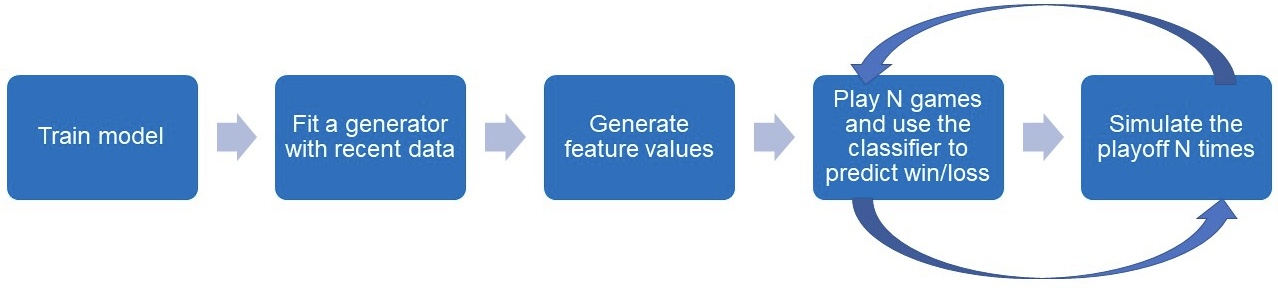
\includegraphics[width=\textwidth]{model/explain.jpeg}} \quad
\label{fig:simulationModel}
\end{figure}
\subsection{Train the classifier}
The goal is to create a function, which, taking two teams as input, returns the winner. To make the winner prediction, it was decided to test three different Machine Learning models, to compare their effectiveness and choose the best one. The Scikit-Learn library ~\cite{Scikit-Learn} in Python was used for the implementation of the models. The \emph{games.csv} dataset was divided by the $70\%$ training set and $30\%$ test set. To train the classifier it has been considered only the match statistics features, 10 in total. The output variable we want to predict is home\_win. Scikit-Learn allows us to use the models without hyperparameterization, so it was decided to make a comparison of the models with and without optimizations. The models have been optimized using the GridSearchCV ~\cite{GridSearchCV} function, which allows us to loop various fittings using combinations of hyperparameters chosen by us. Accuracy and AUC were chosen as metrics to evaluate the models.
\subsubsection{Support Vector Machines}
Using the default values ​​of the Scikit-Learn library  has been obtained an accuracy of $75\%$. It was therefore decided to use GridSearchCV to find the best fitting among the combinations of these parameters: ($C: [0.1, 1, 10], \gamma : [1, 0.5, 0.1, 0.01, 0.001]$, Kernel : [linear, poly, rbf]). The best fit was found for ($C: 0.1, \gamma: 1$, kernel: linear) bringing the accuracy to $83\%$.
\subsubsection{Random Forest}
With the default values, Random Forest obtained an accuracy of $83\%$. So it was decided to try this parameters on GridSearchCV: (n\_estimators: [100, 200, 300, 400, 500], max\_features: [auto, sqrt], max\_depth: [10, 20, 30, 40, 50], bootstrap: [True, False]). The best fit was found for (n\_estimators: 500, max\_features: sqrt, max\_depth: 50, bootstrap: True) but the accuracy remain $83\%$.
\subsubsection{Naive Bayes}
Naive Bayes does not have hyperparameters, and with this model an accuracy of $83\%$ was achieved.
\subsubsection{Area Under the Curve classifiers}
In addition to accuracy, the AUC was also considered, considering the value 1 as a positive label. The higher the AUC value, the better the classifier. Is possible to see that all three models obtained the same performance.
\begin{figure}[h!]
\centering
\subfloat[][Optimize]
{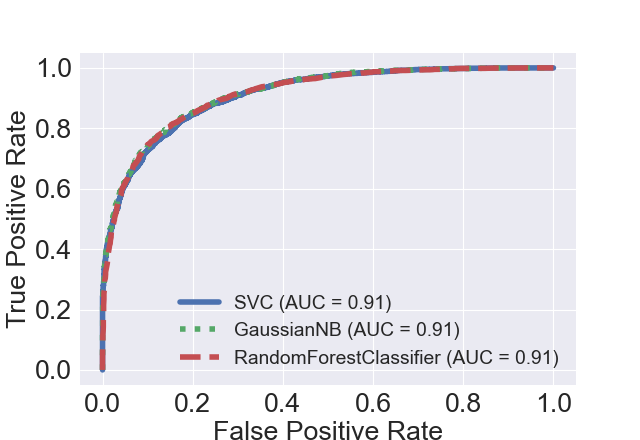
\includegraphics[width=.45\textwidth]{plots/auc_optimize.png}} \quad
\subfloat[][Default]
{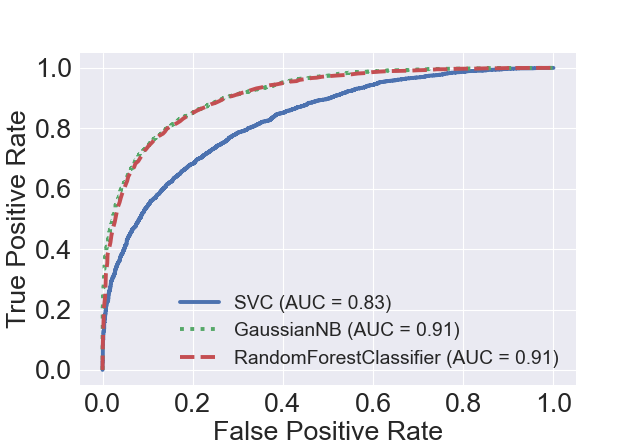
\includegraphics[width=.45\textwidth]{plots/auc_default.png}} \\
\caption{Comparison AUC with and without GridSearchCV}
\label{fig:subfig}
\end{figure}
\label{section: ExperimentalEvaluation}
\subsection{Generate feature values}
To simulate the result of the playoffs it is also necessary to generate possible data on which to predict the future result of the games. To achieve this goal, a \emph{game\_sample} function has been created, which, taken as input two teams, generates possible features of a match. First of all, to create these features, the original dataset was taken considering the most recent data, therefore to predict the 2022 season it was considered from 2020 onwards. For each team it was created a separate datasets with the match statistics results they obtained in each game of \emph{games.csv}, therefore 5 features were taken as we do not distinguish the scores between home or visitor. Using the Fitter ~\cite{Fitter} library available for Python it was possible to obtain the statistical distribution for each of the 5 features for each team. The \emph{game\_sample} function in the simulator therefore generates a random sample of features from the distribution for each of the two input teams and by putting the features together it is possible to generate a possible result of a match between the two teams.
\subsection{Simulate playoff}
The simulator takes as input the list of teams admitted to the playoffs and is composed of three functions: (\emph{play\_ngames, play\_round, simulate}). The \emph{play\_ngames} function takes two teams as input and generates a sample of features using \emph{game\_sample} for each of the 7 games, the result for each game is predicted using the classifier. In the \emph{play\_round} function, \emph{play\_ngames} is repeated for each round, eliminating the eliminated teams from the list. Finally, to get a statistic and return a probability in the \emph{simulate} function, $N$ iterations of \emph{play\_round} are made and for each round of the playoffs it is kept track of the times in which a team has managed to pass to the next round. Therefore the final result of the simulation is the probability that a team has to move on to the next round.
\subsection{Results and discussion}
\label{ResultsAndDiscussion}
The figure below shows the output achieved after 5000 simulations of the playoffs of the current season 2021-2022, using Random Forest as a classifier. It is possible to see that with the exception of the Suns-Mavericks, Bucks-Celtics and Heat-Celtics matches, the rest was correctly predicted. The reason for the mistake can be admitted to the fact that Suns and Bucks played below expectations, Heat and Celtics was a very tight match and in general Celtics played beyond expectations, however the winner of the finals was correctly predicted. These predictions could be further improved by adding player statistics, injuries, or match strategies used in previous matches.  
\begin{figure}[h!]
\centering
\subfloat[][playoffs]
{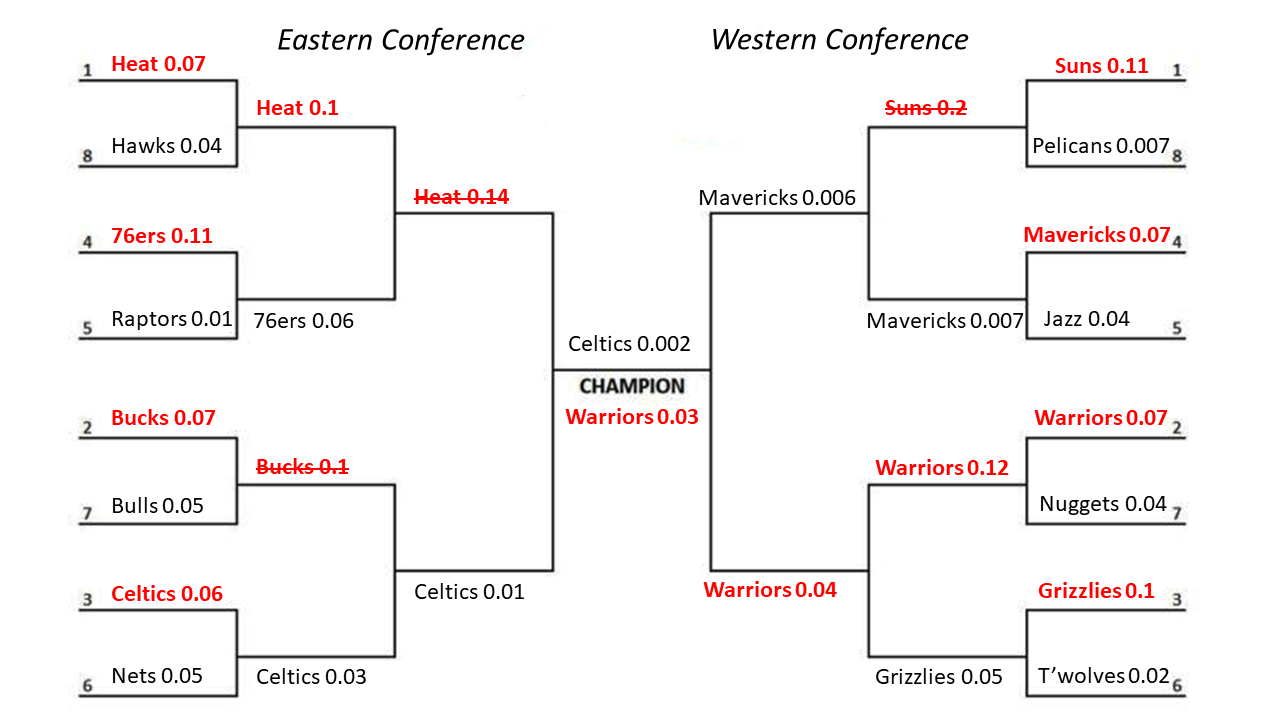
\includegraphics[width=\textwidth]{model/playoffs.png}} \quad
\label{fig:playoffs}
\end{figure} 

\bibliographystyle{plain}
\bibliography{bibliography}
\end{document}
